
 \newpage
\subsection{SPI Interface}
This section describes the protocol used to communicate with the chip.

\begin{figure}[H]
\centering
\captionsetup{justification=centering}
\includegraphics[scale=0.35]{../figures/spi_data.png}
\caption{SPI data diagram}
\label{data}
\end{figure}

As an attempt to save time on implementation, the group decided to deviate from the standard spi protocol and create an specialized protocol for the chip.\\
The total amount of data that should be sent, during each active period of SPI_enable, is 4 x 4 16 bit words to the chip and four 17 bit words from the chip. This is illustrated in Fig. \ref{spi_data}.
The chip receive and send data with the most significant bit first. The order of the bits is illustrated Fig. \ref{spi_int}. \\

\begin{figure}[H]
\centering
\captionsetup{justification=centering}
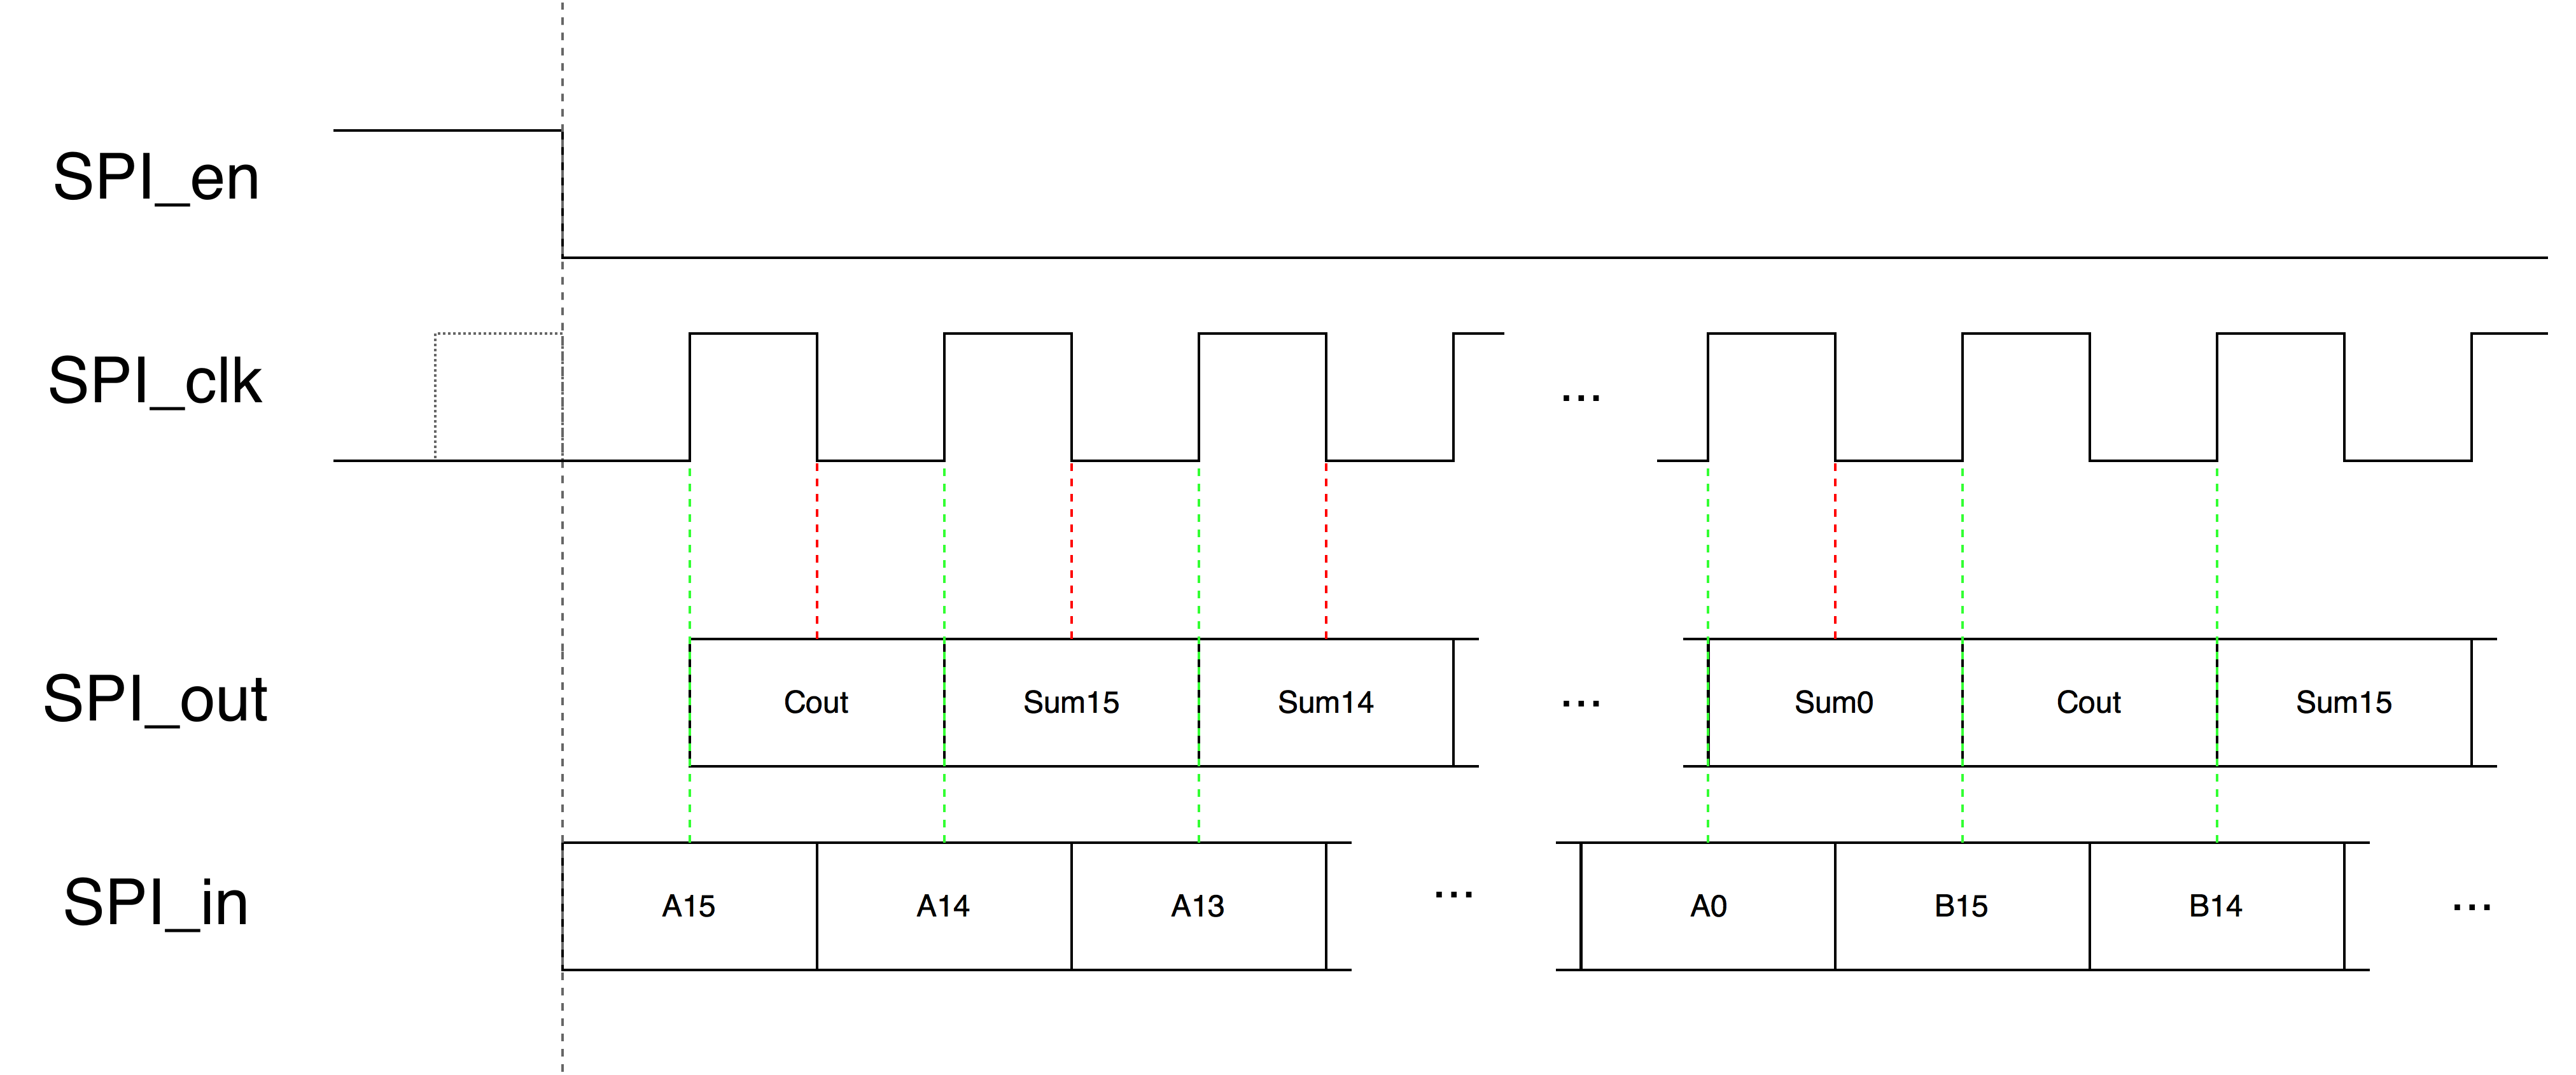
\includegraphics[scale=0.35]{../figures/spi_interface.png}
\caption{SPI timing diagram}
\label{spi_int}
\end{figure}

Data is both written and read by the chip on the rising edge of the the spi clock. This means that the circuitry communicating with the chip has to read and write on the falling edge of the clock. The first input data should be available on the first rising edge after SPI_en goes low, and the first bit of the output will be available on the first falling edge after spi enable goes low. This can also be seen in Fig. \ref{spi_int}

\begin{figure}[H]
\centering
\captionsetup{justification=centering}
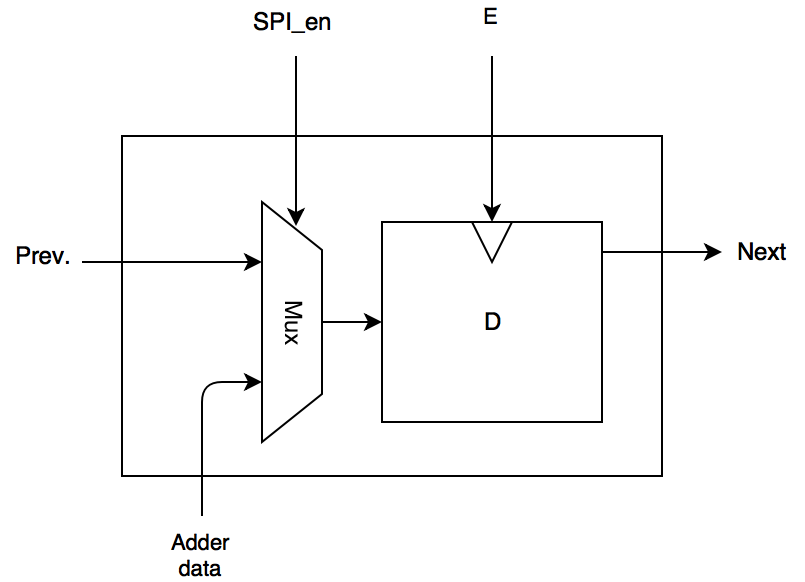
\includegraphics[scale=0.35]{../figures/MUX_DFF.png}
\caption{Shift register cell}
\label{mux_dff}
\end{figure}